
%(BEGIN_QUESTION)
% Copyright 2010, Tony R. Kuphaldt, released under the Creative Commons Attribution License (v 1.0)
% This means you may do almost anything with this work of mine, so long as you give me proper credit

Skisser tilkoblingsledninger som viser hvordan du simulerer et \textit{RTD}-signal til inngangen på denne elektroniske temperaturtransmitteren ved bruk av et potensiometer:

$$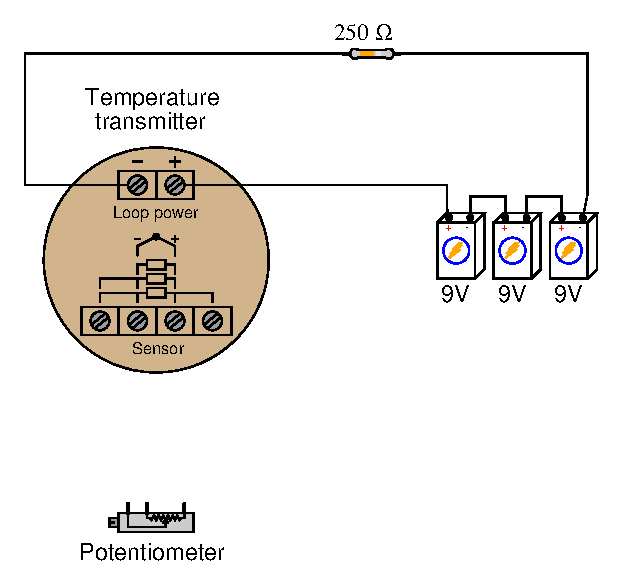
\includegraphics[width=15.5cm]{i00251x01.eps}$$

Anta at transmitteren er riktig konfigurert for {\bf 2-leder} RTD-inngang, og at potensiometeret har tilstrekkelig presisjon og oppløsning slik at det ikke er nødvendig å koble det sammen med andre motstander i et nettverk.

\underbar{file i00251}
%(END_QUESTION)





%(BEGIN_ANSWER)

$$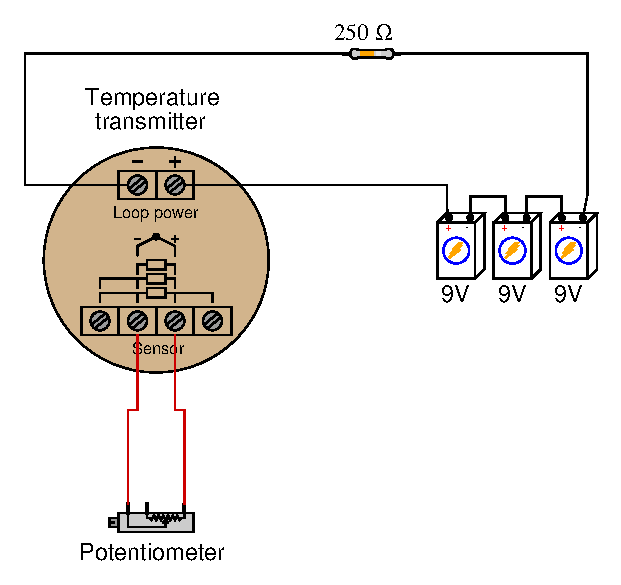
\includegraphics[width=15.5cm]{i00251x02.eps}$$

Alle korrekte løsninger vil ha disse egenskapene:

\begin{itemize}
\item{} Potensiometer koblet som reostat (kun sleider og én annen terminal brukt, eventuelt tredje terminal koblet felles med sleider)
\item{} Én leder fra transmitter til sleider
\item{} Én leder fra transmitter til den andre reostat-terminalen
\end{itemize}

%(END_ANSWER)





%(BEGIN_NOTES)

{\bf This question is intended for exams only and not worksheets!}.

%(END_NOTES)
